\documentclass[12pt,letterpaper]{article}

\usepackage{amsmath, amsthm}
\usepackage{microtype, parskip}
\usepackage[comma,numbers,sort&compress]{natbib}
\usepackage{lineno}
\usepackage{docmute}
\usepackage{caption, subcaption, multirow, morefloats, rotating}
\usepackage{wrapfig}

\frenchspacing

\captionsetup[subfigure]{position = top, labelfont = bf, textfont = normalfont, singlelinecheck = off, justification = raggedright}

\begin{document}
\section{Results}

As stated above, posterior approximations for both the exponential and Weibull models achieved approximate stationarity after 10,000 steps, as all parameter estimates have an \(\hat{R} < 1.1\).%\uppercase{ref tables}.

Comparisons of the survival functions estimated from 1000 posterior predictive data sets to the estimated survival function of the observed genera demonstrates that both the exponential and Weibull models approximately capture the observed pattern of extinction (Fig. \ref{fig:surv}). The major difference in fit between the two models is that the Weibull model has a slightly better fit for longer lived taxa than the exponential model.

%Inspection of the deviance residuals yields a similar pattern of biased estimates for longer lived taxa \uppercase{ref figure}. 

Additionally, the Weibull model is expected to have slightly better out-of-sample predictive accuracy when compared to the exponential model (WAIC 4576 versus 4604, respectively). \ref{fig:surv}). Because the difference in WAIC between these two models is large, while results from both the exponential and Weibull models will be presented, only those from the Weibull model will be discussed.

% Results/hypothesis tests
%   \mu of hierarchical effects
%   \tau of hierarchical effects (partial pooling)
Estimates of the overall mean covariate effects \(\mu\) can be considered time-invariant generalizations for brachiopod survival during the Paleozoic (Fig. \ref{tab:param}). Consistent with prior expectations, geographic range size has a negative effect on extinction risk, where genera with large ranges having greater durations than genera with small ranges. 

I find that while the mean estimate of the effect of body size on extinction risk is negative, implying that increasing body size decreases extinction risk, this estimate is within 2 standard deviations of 0 (mean \(\mu_{m} = -0.09\), standard deviation 0.09; Fig. \ref{tab:param}). Because of this, I infer that body size has no distinguishable effect on brachiopod taxonomic survival.

Interpretation of the effect of environmental preference \(v\) on duration is slightly more involved. Because a quadratic term is the equivalent of an interaction term, both \(\mu_{v}\) and \(\mu_{v^{2}}\) have to be interpreted together because it is illogical to change values of \(v\) without also changing values \(v^{2}\). To determine the nature of the effect of \(v\) on duration I calculated the multiplicative effect of environmental preference on extinction risk.

Given mean estimated extinction risk \(\tilde{\sigma}\), we can define the extinction risk multiplier of an observation with environmental preference \(v_{i}\) as 
\begin{equation}
  \frac{\tilde{\sigma_{i}}}{\tilde{\sigma}} = f(v_{i}) = \exp\left(\frac{-(\mu_{v} v_{i} + \mu_{v^{2}} v^{2})}{\alpha}\right).
  \label{eq:env}
\end{equation}
This function \(f(v_{i})\) has a y-intercept of \(\exp(0)\) or 1 because it does not have a non-zero intercept term. Equation \ref{eq:env} can be either concave up or down. A concave down \(f(v_{i})\) may indicate that genera of intermediate environmental preference have greater durations than either extreme, and \textit{vice versa} for concave up function.

The expected effect of environmental preference as a multiplier of expected extinction risk can then be visualized (Fig. \ref{fig:env_mean}). This figure depicts 1000 posterior predictive estimates of Eq. \ref{eq:env} across all possible values of \(v\). The number indicates the posterior probability that the function is concave down, with generalists having lower extinction risk/greater duration than either type of specialist. Note that the inflection point/optimum of Fig. \ref{fig:env_mean} is approximately \(x = 0\), something that is expected given the estimate of \(\mu_{v}\) (Fig. \ref{tab:param}).

The matrix \(\Sigma\) describing the covariance between the different coefficients describes how these coefficients might vary together across the origination cohorts. Similar to how this was modeled (Eq. \ref{eq:exp_total}, \ref{eq:wei_total}), for interpretation purposes \(\Sigma\) can be decomposed into a vector of standard deviations \(\vec{\tau}\) and a correlation matrix \(\Omega\).

The estimates of the standard deviation of between-cohort coefficient estimates \(\tau\) inidicate that some effects can vary greatly between-cohorts (Fig. \ref{tab:param}). Coefficients with greater values of \(\tau\) have greater between-cohort variation. The covariate effects with the greatest between origination cohort variation are \(\beta_{r}\), \(\beta_{v}\), and \(\beta_{v^{2}}\). Estimates of \(\beta_{m}\) have negligible between cohort variation, as there is less between cohort variation than the between cohort variation in baseline extinction risk \(\beta_{0}\). However the amount of between cohort variation in estimates of \(\beta_{v^{2}}\) means that it is possible for the function describing the effect of environmental affinity to be upward facing for some cohorts (Eq. \ref{eq:env}), which corresponds to environmental generalists being shorter lived than specialists in that cohort.


% omega heatmap
%   correlations with baseline extinction risk of of major interest
%   high/positive values of intercept --> high extinction risk
%   low/negative values of intercept --> low extinction risk
The correlation terms of \(\Omega\) (Fig. \ref{fig:omega}) describe the relationship between the coefficients and how their estimates may vary together across cohorts. The correlations between the intercept term \(\beta_{0}\) and the effects of the taxon traits are of particular interest for evaluating the \citet{Jablonski1986} scenario (Fig. \ref{fig:omega} first column/last row). Keep in mind that when \(\beta_{0}\) is low, extinction risk is low; and conversely, when \(\beta_{0}\) is high, then extinction risk is high.

Marginal posterior probabilities of the correlations between the level of baseline extinction risk \(\beta_{0}\) and the effects of the taxon traits indicate that the correlation between expected extinction risk and both geographic range \(\beta_{r}\) and \(\beta_{v^{2}}\) are of particular note (Fig. \ref{fig:corr}). 

There is approximately a 98\% probability that \(\beta_{0}\) and \(\beta_{r}\) are negatively correlated (Fig. \ref{fig:corr}), meaning that as extinction risk increases, the effect/importance of geographic range on genus duration increases. This means that increases in baseline extinction rate are correlated with an increased importance of geographic range size. There is a 93\% probability that \(\beta_{0}\) and \(\beta_{v^{2}}\) are negatively correlated (Fig. \ref{fig:corr}), meaning that as extinction risk increases, the peakedness of \(f(v_{i})\) increases and the relationship tends towards concave down. Additionally, there is a 97\% probability that values of \(\beta_{r}\) and \(\beta_{v^{2}}\) are positively correlated (Mean correlation 0.51, standard deviation 0.23).

% effects varying between cohorts
While the overall group level estimates are of particular importance when defining time-invariant differences in extinction risk, it is also important and useful to analyze the individual level parameter estimates in order to better understand how parameters actually vary across cohorts.

In comparison to the overall mean extinction risk \(\mu_{0}\), cohort level estimates \(\beta_{0}\) show some amount of variation through time as expected by estimates of \(\tau_{0}\) (Fig. \ref{fig:cohort_intercept}). A similar, if slightly greater, amount of variation is also observable in cohort estimates of the effect of geographic range \(\beta_{r}\) (Fig. \ref{fig:cohort_range}). Again, smaller values of \(\beta_{0}\) correspond to lower expected extinction risk. Similarly, smaller values of \(\beta_{r}\) correspond to greater decrease in extinction risk with increasing geographic range 

% environmental effect for cohort
%   effect of environmental preference as duration multiplier
How the effect of environmental affinity varies between cohorts can be observed by using the cohort specific coefficients estimates. Following the same procedure used earlier (Fig. \ref{tab:param}), but substituting cohort specific estimates of \(\beta_{v}\) and \(\beta_{v^{2}}\) for \(\mu_{v}\) and \(\mu_{v^{2}}\), the cohort specific effect of environmental preference as a multiplier of mean extinction risk can be calculated. This was done only for the Weibull model, though the observed pattern should be similar for the exponential model. 

As expected based on the estimates of \(\tau_{v}\) and \(\tau_{v^{2}}\), there is greater variation in the peakedness of \(f(v_{i})\) than there is variation between convave up and down functions (Fig. \ref{fig:env_cohort}). 12 of the 33 cohorts have less than 50\% posterior probability that generalists are potentially expected to be shorter lived than specialists, though two of those cases have approximately a 50\% probability of being either concave up or down. This is congruent with the 0.72 posterior probability that \(\mu_{v^{2}}\) is positive/\(f(v_{i})\) is concave down.


Additionally, for some cohorts there is a quite striking pattern where the effect of environmental preference \(v\) has a nearly-linear relationship (Fig. \ref{fig:env_cohort}). These are primarily scenarios where one of the end member preferences is expected to have a greater duration than either intermediate or the opposite end member preference. Whatever curvature is present in these nearly-linear cases is due to the defintion of \(f(v)\) as it is not defined for non-negative values of \(\sigma\) (Eq. \ref{eq:env}). For all stages between the Emsian through the Vis\'{e}an, inclusive, intermediate preferences are of intermediate extinction risk when compared with epicontinental specialists (lowest risk) or open-ocean specialists (highest risk). This time period represents most of the Devonian through the early Carboniferous.

\begin{figure}[ht]
  \centering
  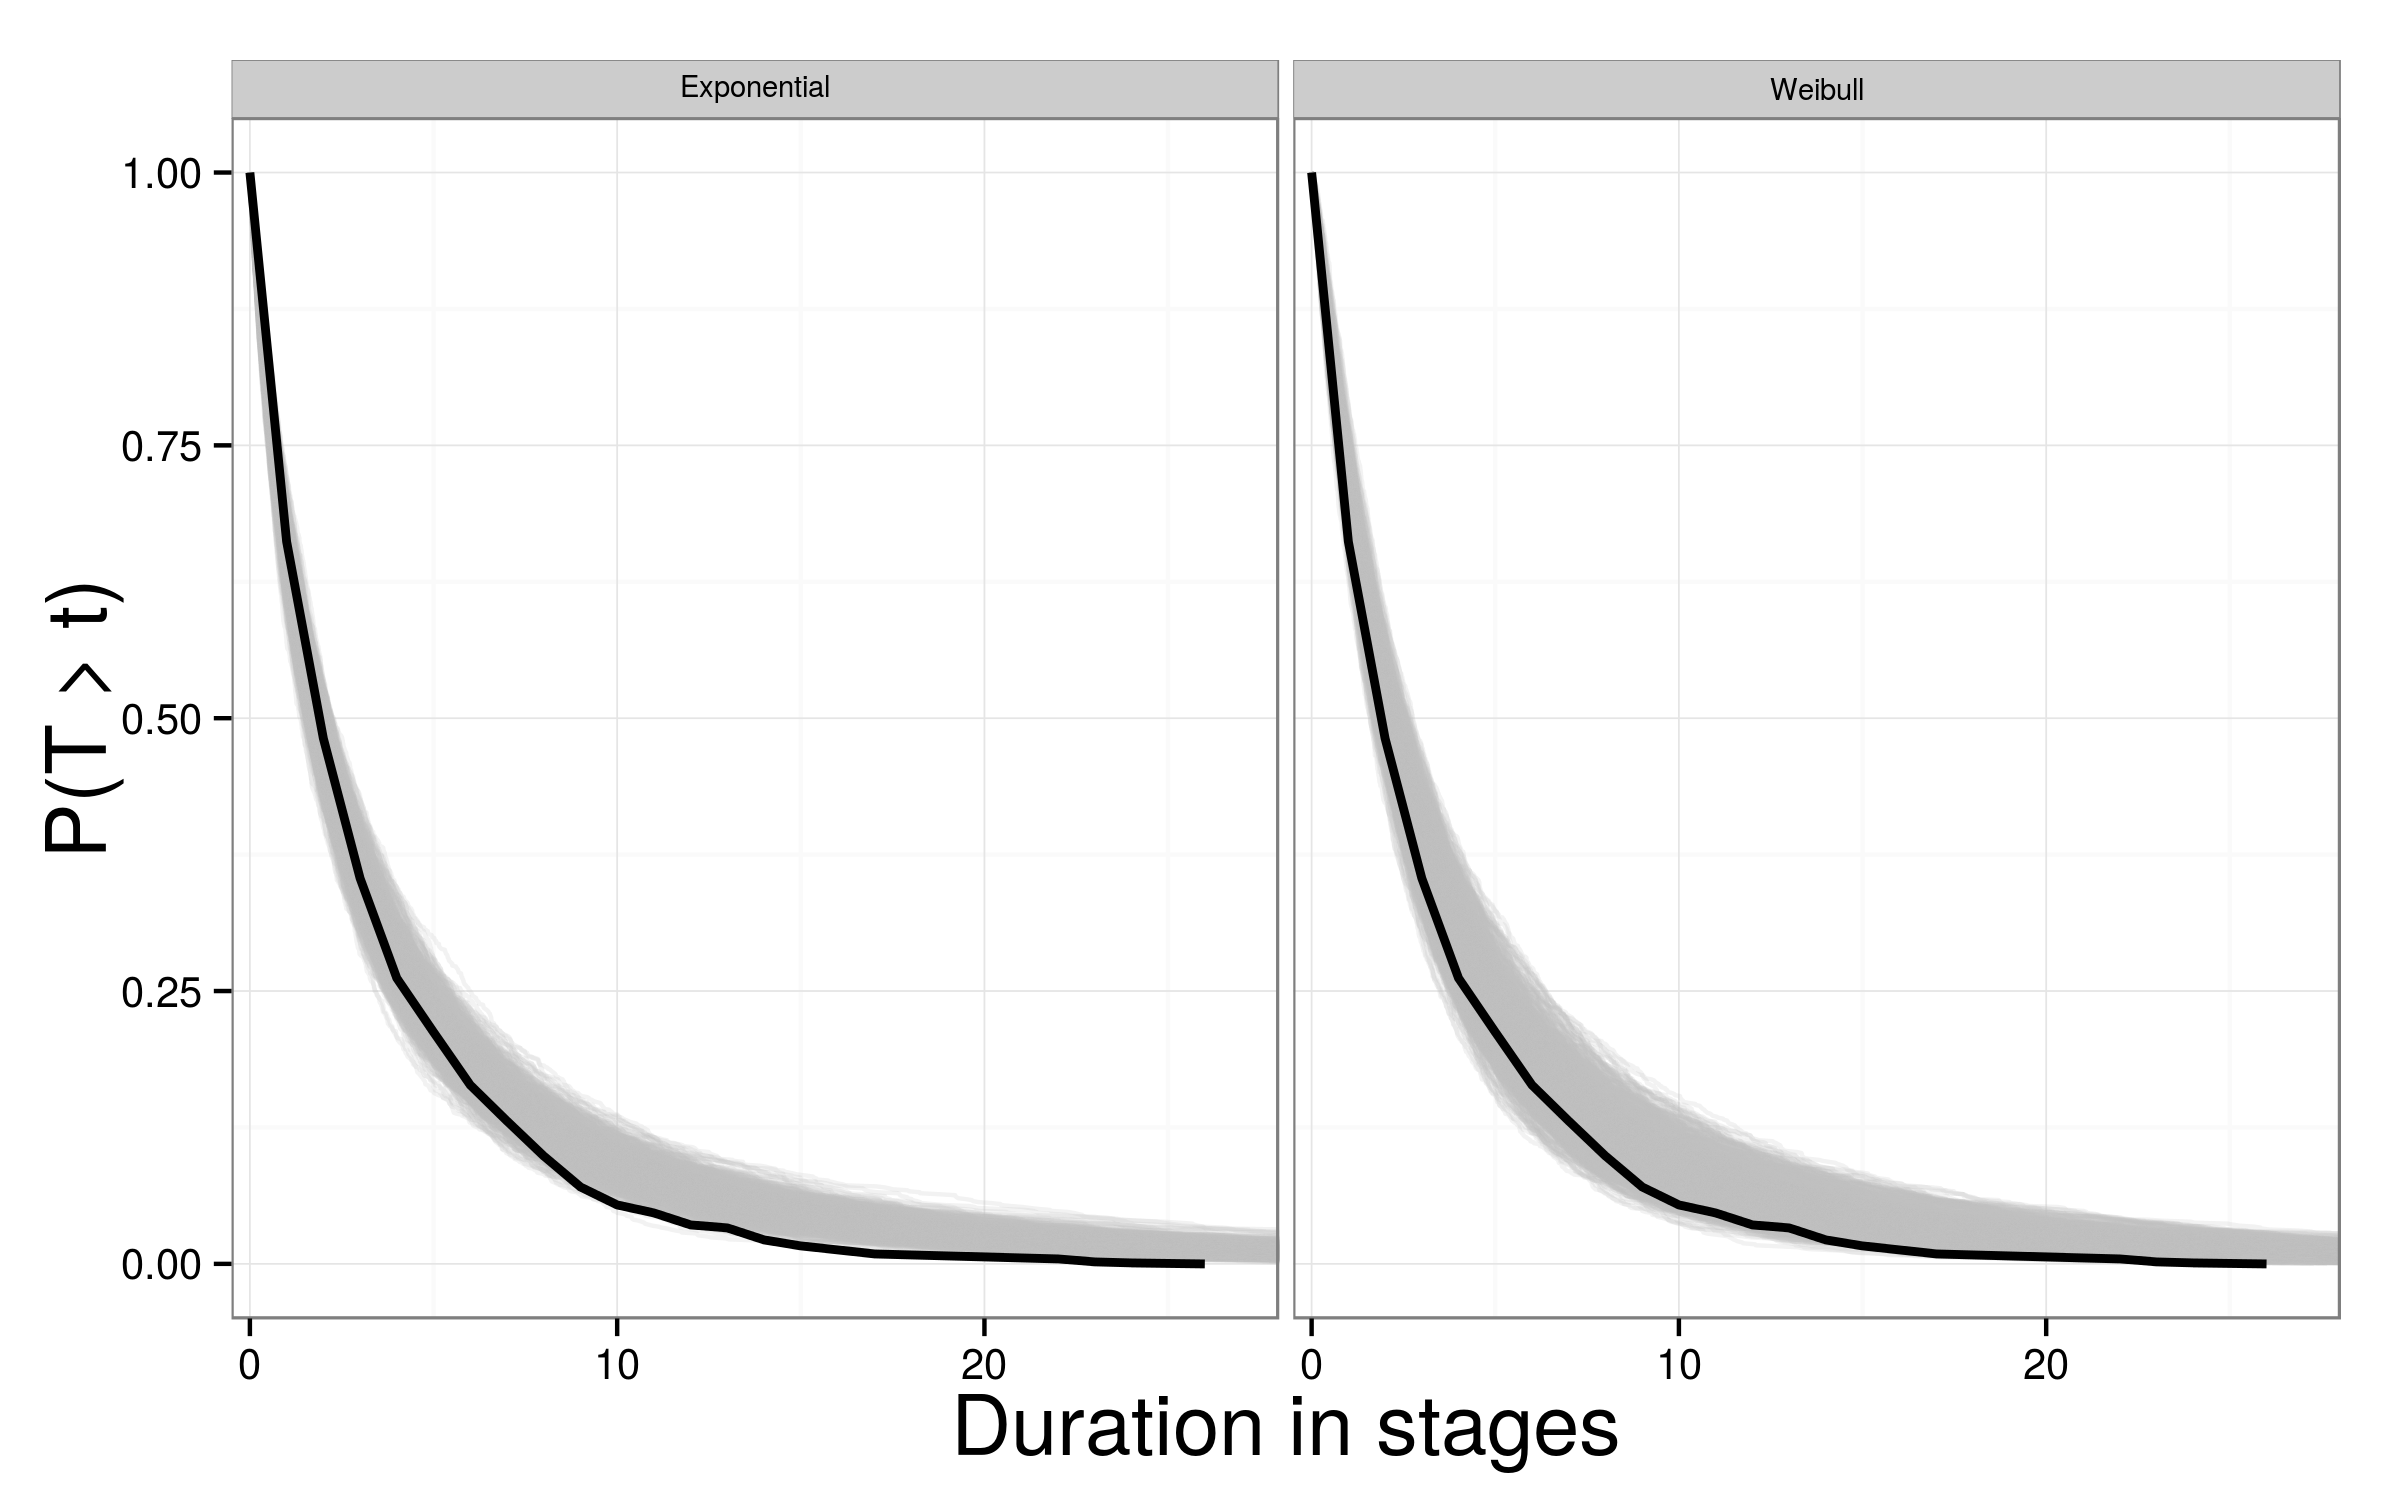
\includegraphics[height = 0.5\textheight,width=\textwidth,keepaspectratio=true]{figure/survival_curves}
  \caption{Comparison of empirical estimates of \(S(t)\) versus estimates from 1000 posterior predictive data sets. \(S(t)\) corresponds to \(P(T > t)\) as it is the probability that a given genus observed at age \(t\) will continue to live. This is equivalent to the probability that \(t\) is less than the genus' ultimate duration \(T\). Note that the Weibull (left) model has noticeably better fit to the data than the exponential (right).}
  \label{fig:surv}
\end{figure}

\begin{figure}[ht]
  \centering
  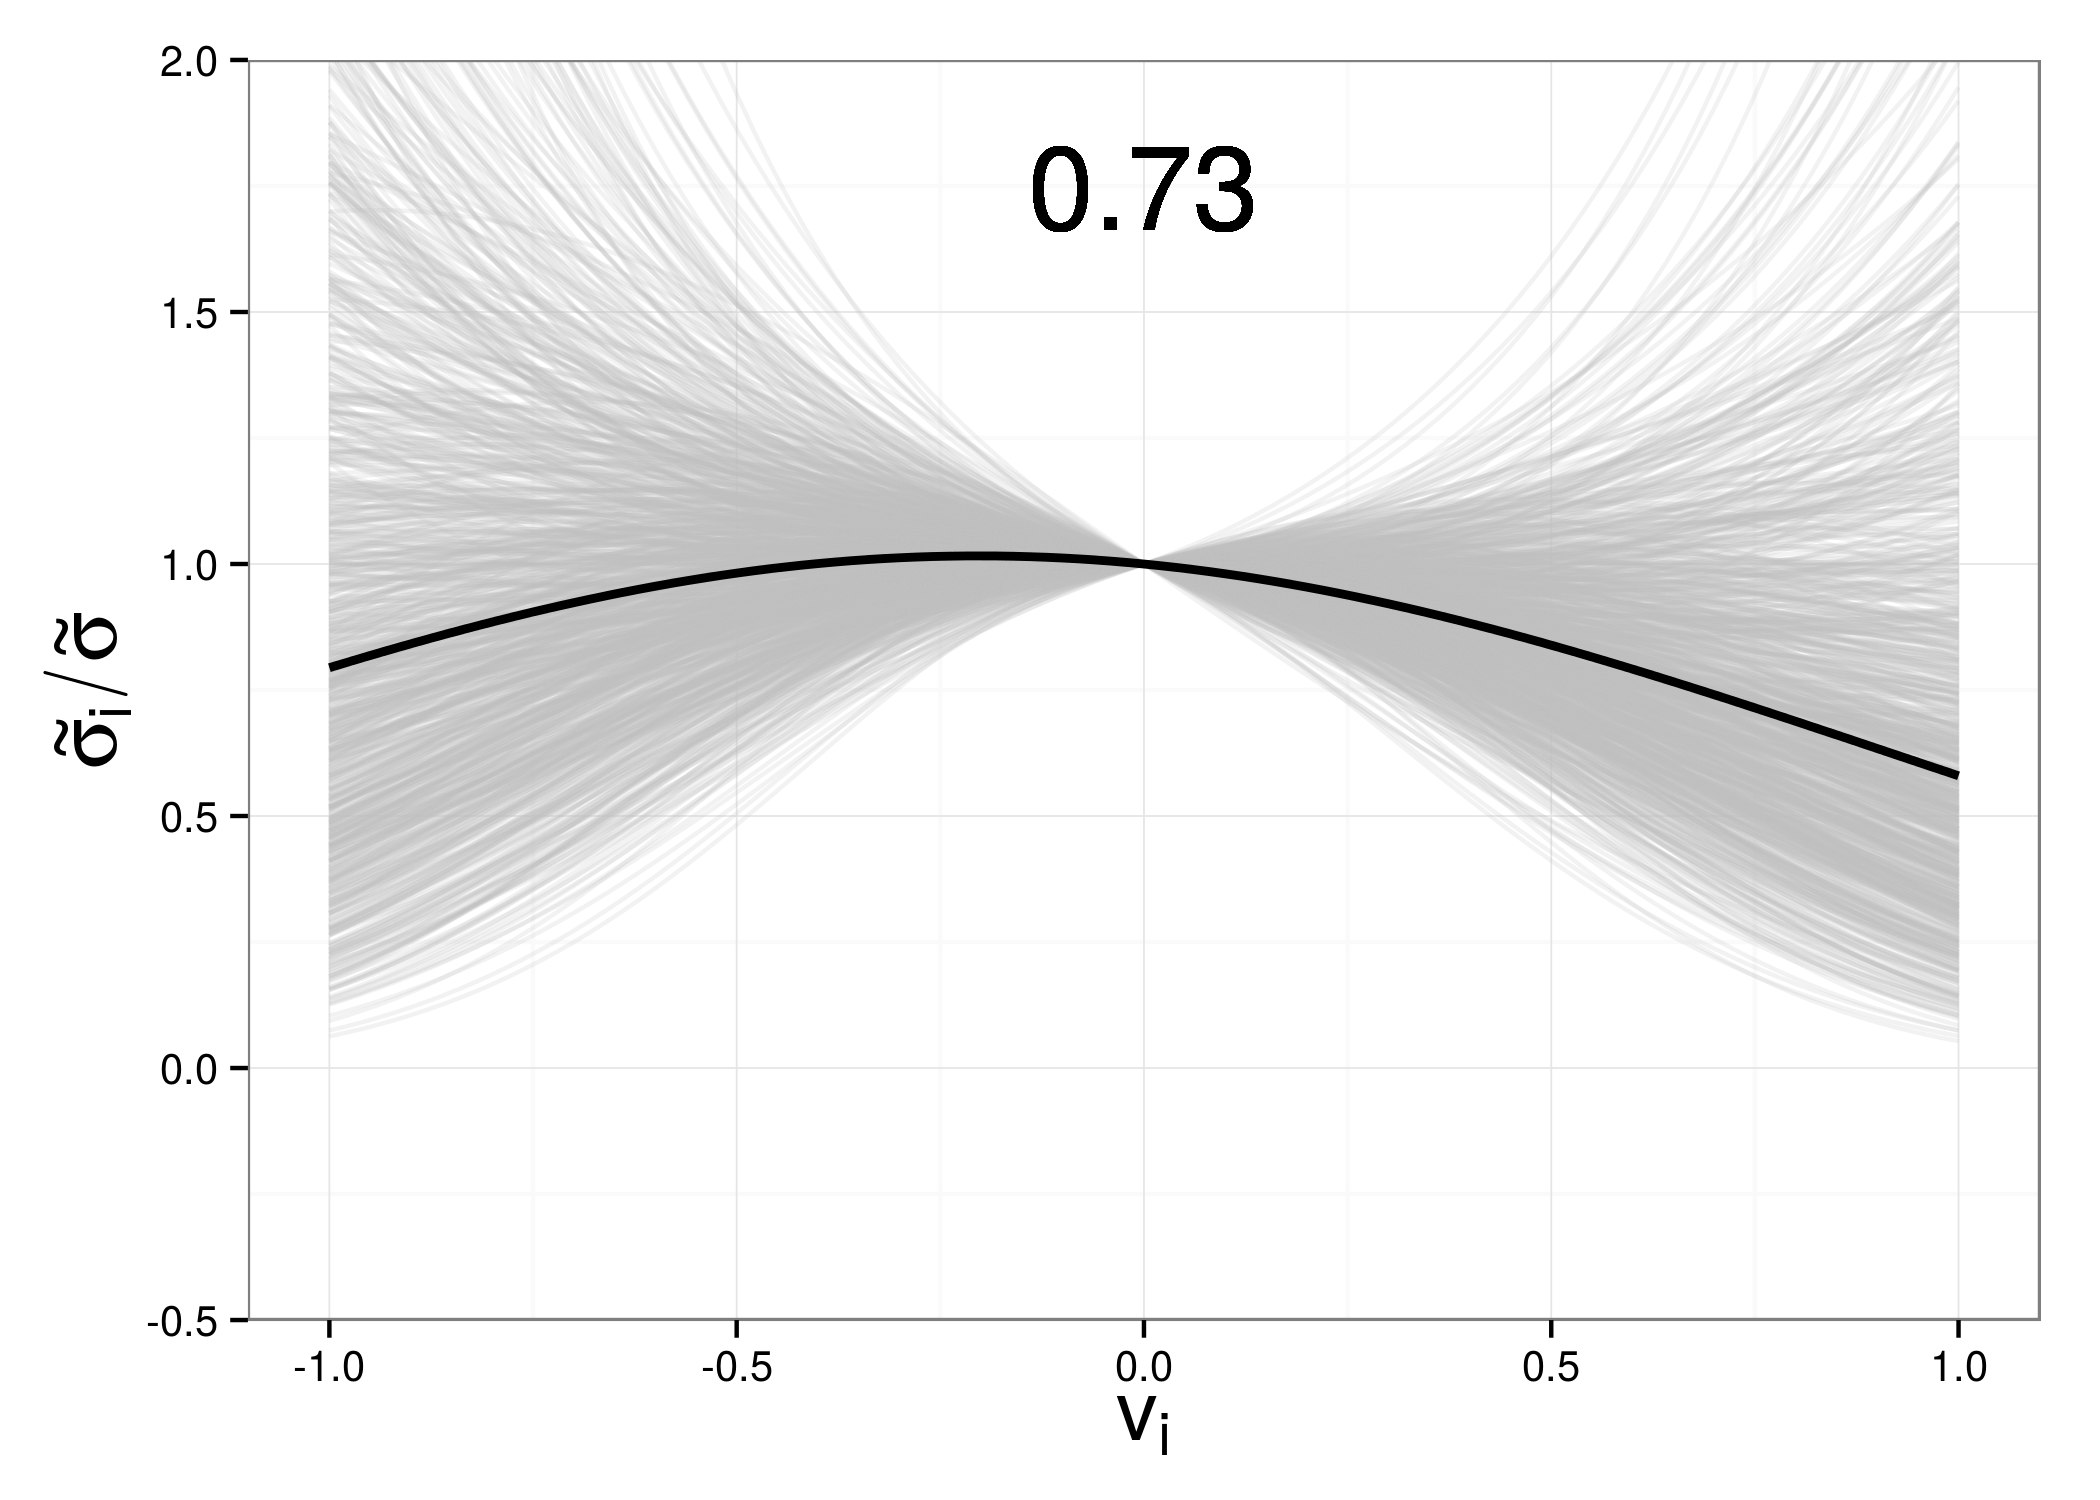
\includegraphics[height = 0.5\textheight,width=\textwidth,keepaspectratio=true]{figure/environ_quad}
  \caption{The overall expected relationship \(f(v_{i})\) between environmental affinity \(v_{i}\) and a multiplier of extinction risk (Eq. \ref{eq:env}). Each grey line corresponds to a single draw from the posterior predictive distribution, while the black corresponds to the median of the posterior predictive distribution. The overall shape of \(f(v_{i})\) is concave down with an optimum of close 0, which corresponds to affinity approximately equal to the expectation based on background environmental occurrence rates.}
  \label{fig:env_mean}
\end{figure}


\begin{figure}[ht]
  \centering
  \begin{subfigure}[b]{0.5\textwidth}
    \caption{}
    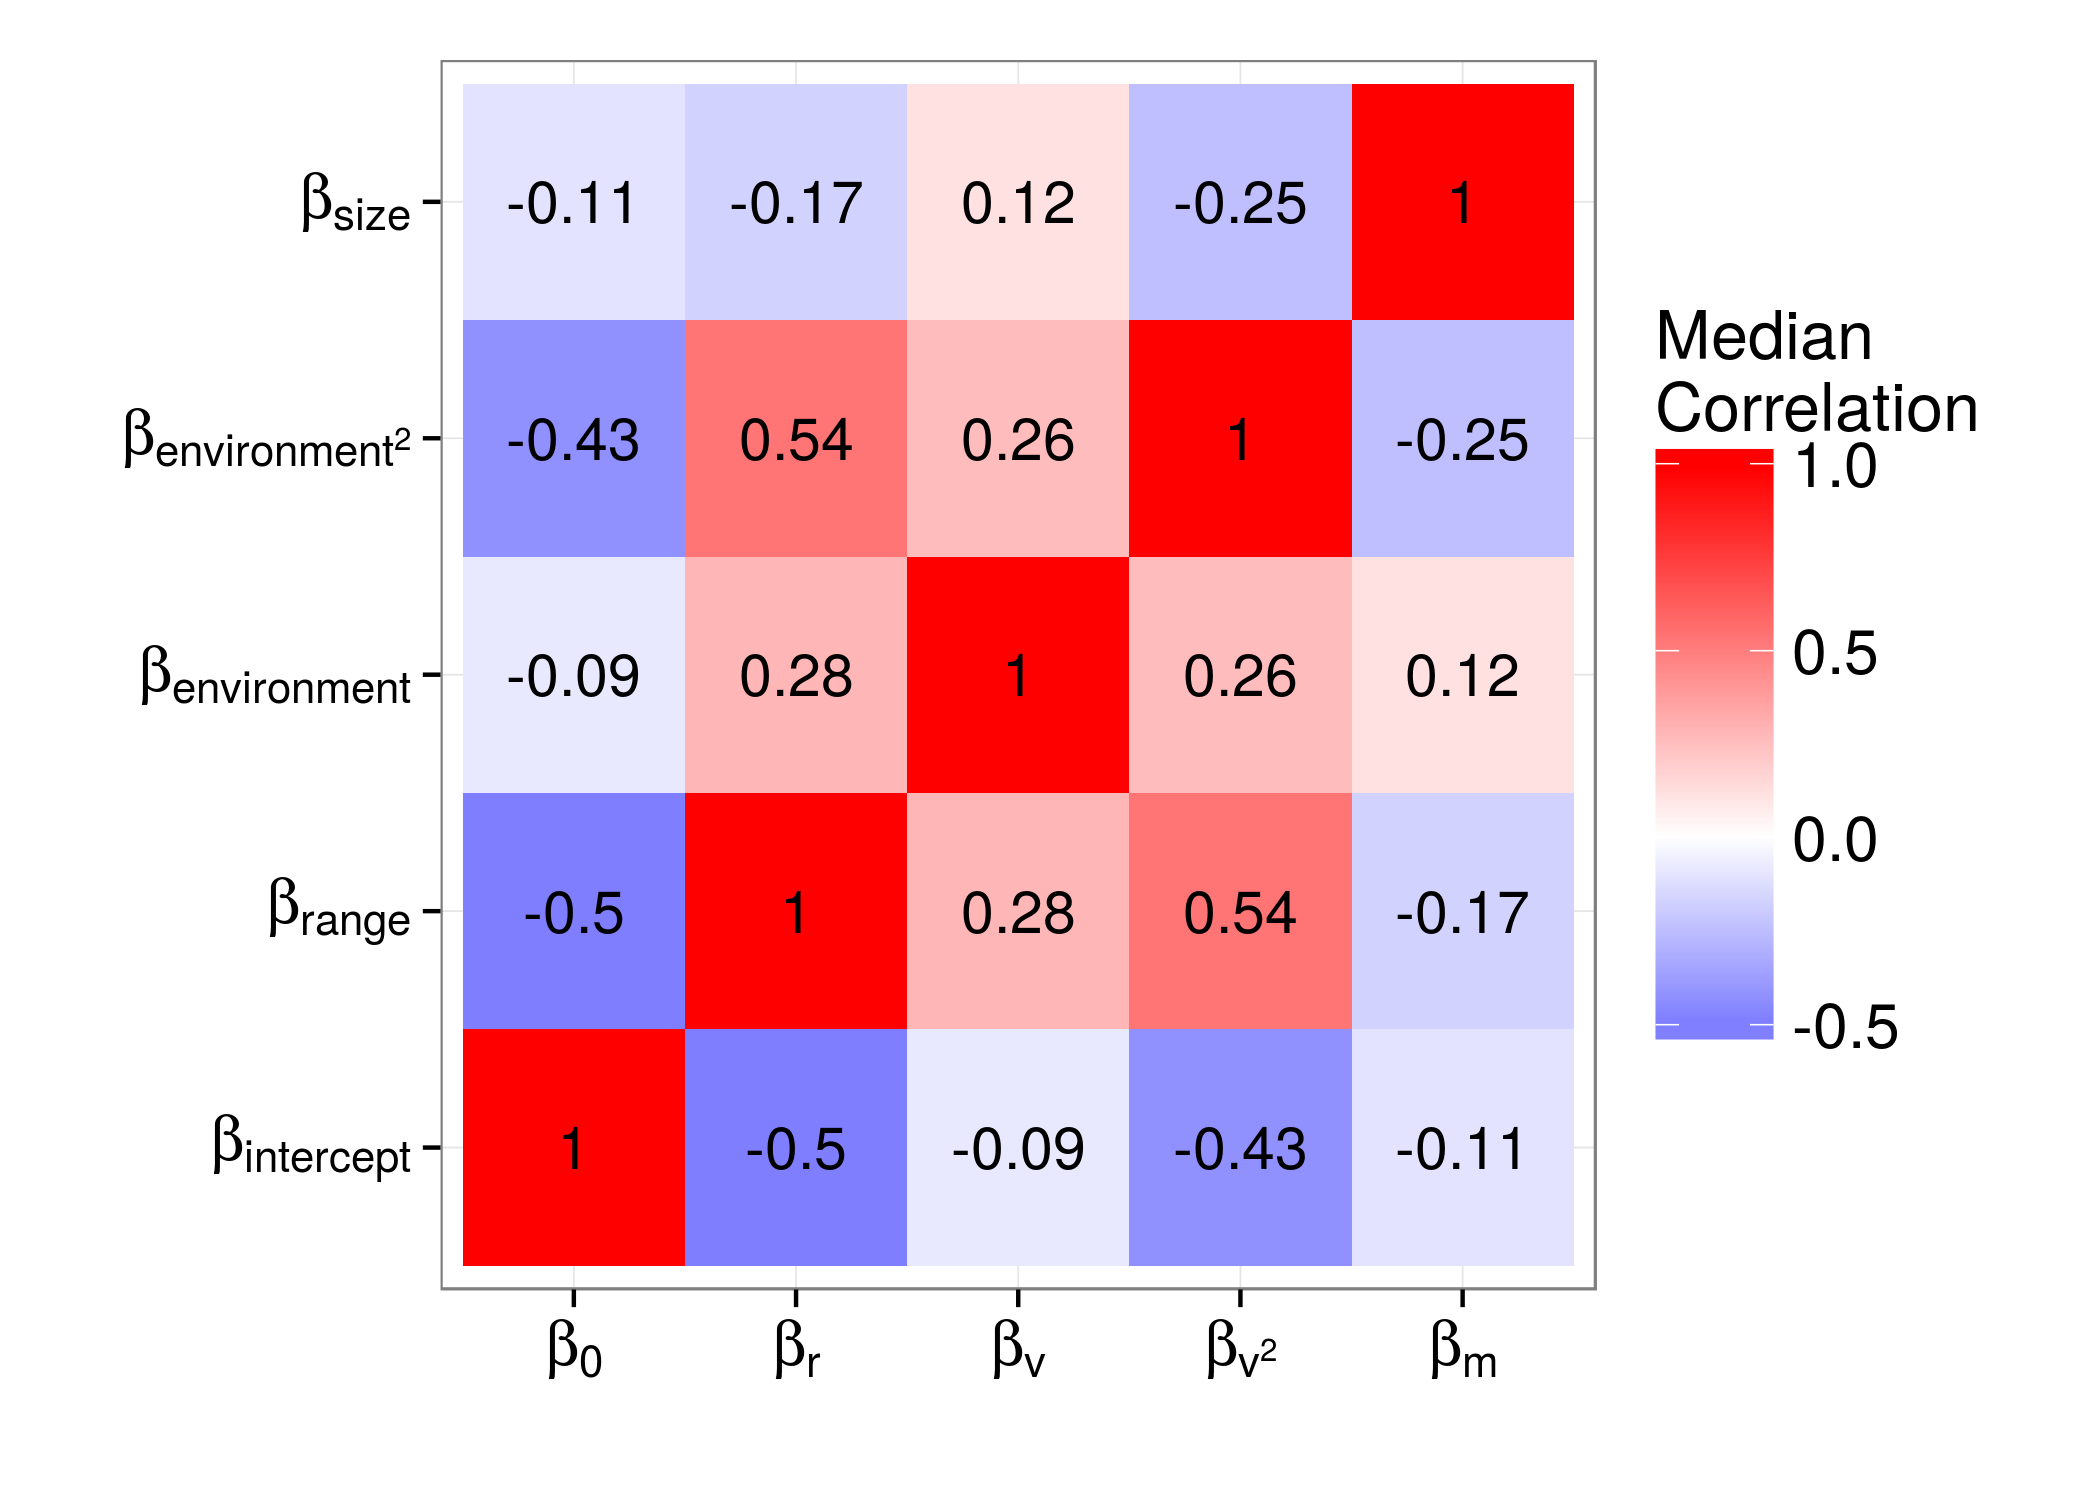
\includegraphics[height = 0.5\textheight,width=\textwidth,keepaspectratio=true]{figure/wei_cor_heatmap}
    \label{fig:omega}
  \end{subfigure}
  \begin{subfigure}[b]{0.4\textwidth}
    \caption{}
    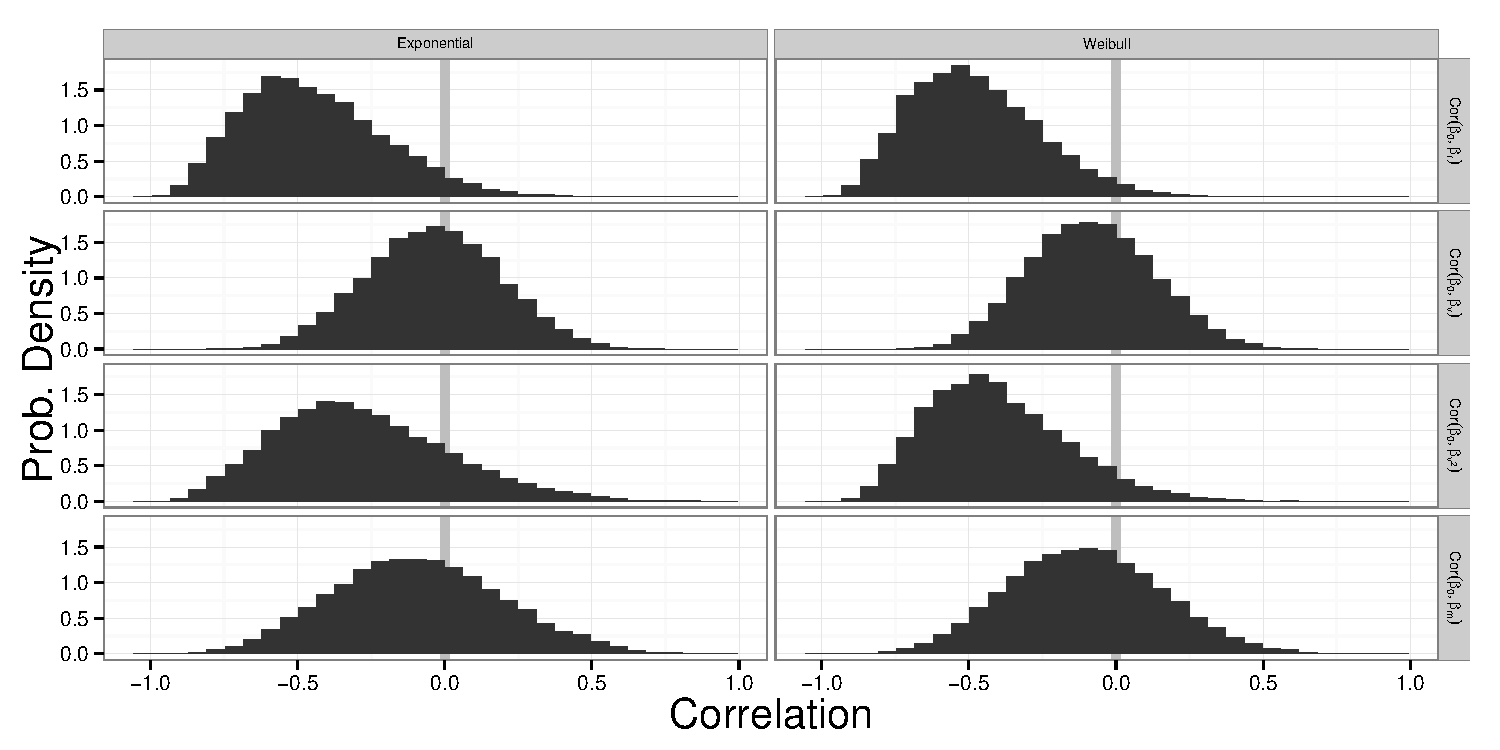
\includegraphics[height = 0.5\textheight,width=\textwidth,keepaspectratio=true]{figure/correlation_marginal}
    \label{fig:corr}
  \end{subfigure}
  \caption{\textbf{A}: Heatmap for the median estimates of the terms of the correlation matrix \(\Omega\) between cohort-level covariate effects. Both the exponential (left) and Weibull (right) models are presented. The off-diagonal terms are the correlation between the estimates of the cohort-level estimates of the effects of covariates, along with intercept/baseline extinction risk. \textbf{B}: Marginal posterior distributions of the correlations between intercept terms/baseline extinction risk and the effects of each of the covariates. These are presented for both the exponential (left) and Weibull (right) models.}
  \label{fig:cor_posterior}
\end{figure}


\begin{figure}[ht]
  \centering
  \begin{subfigure}[b]{\textwidth}
    \caption{}
    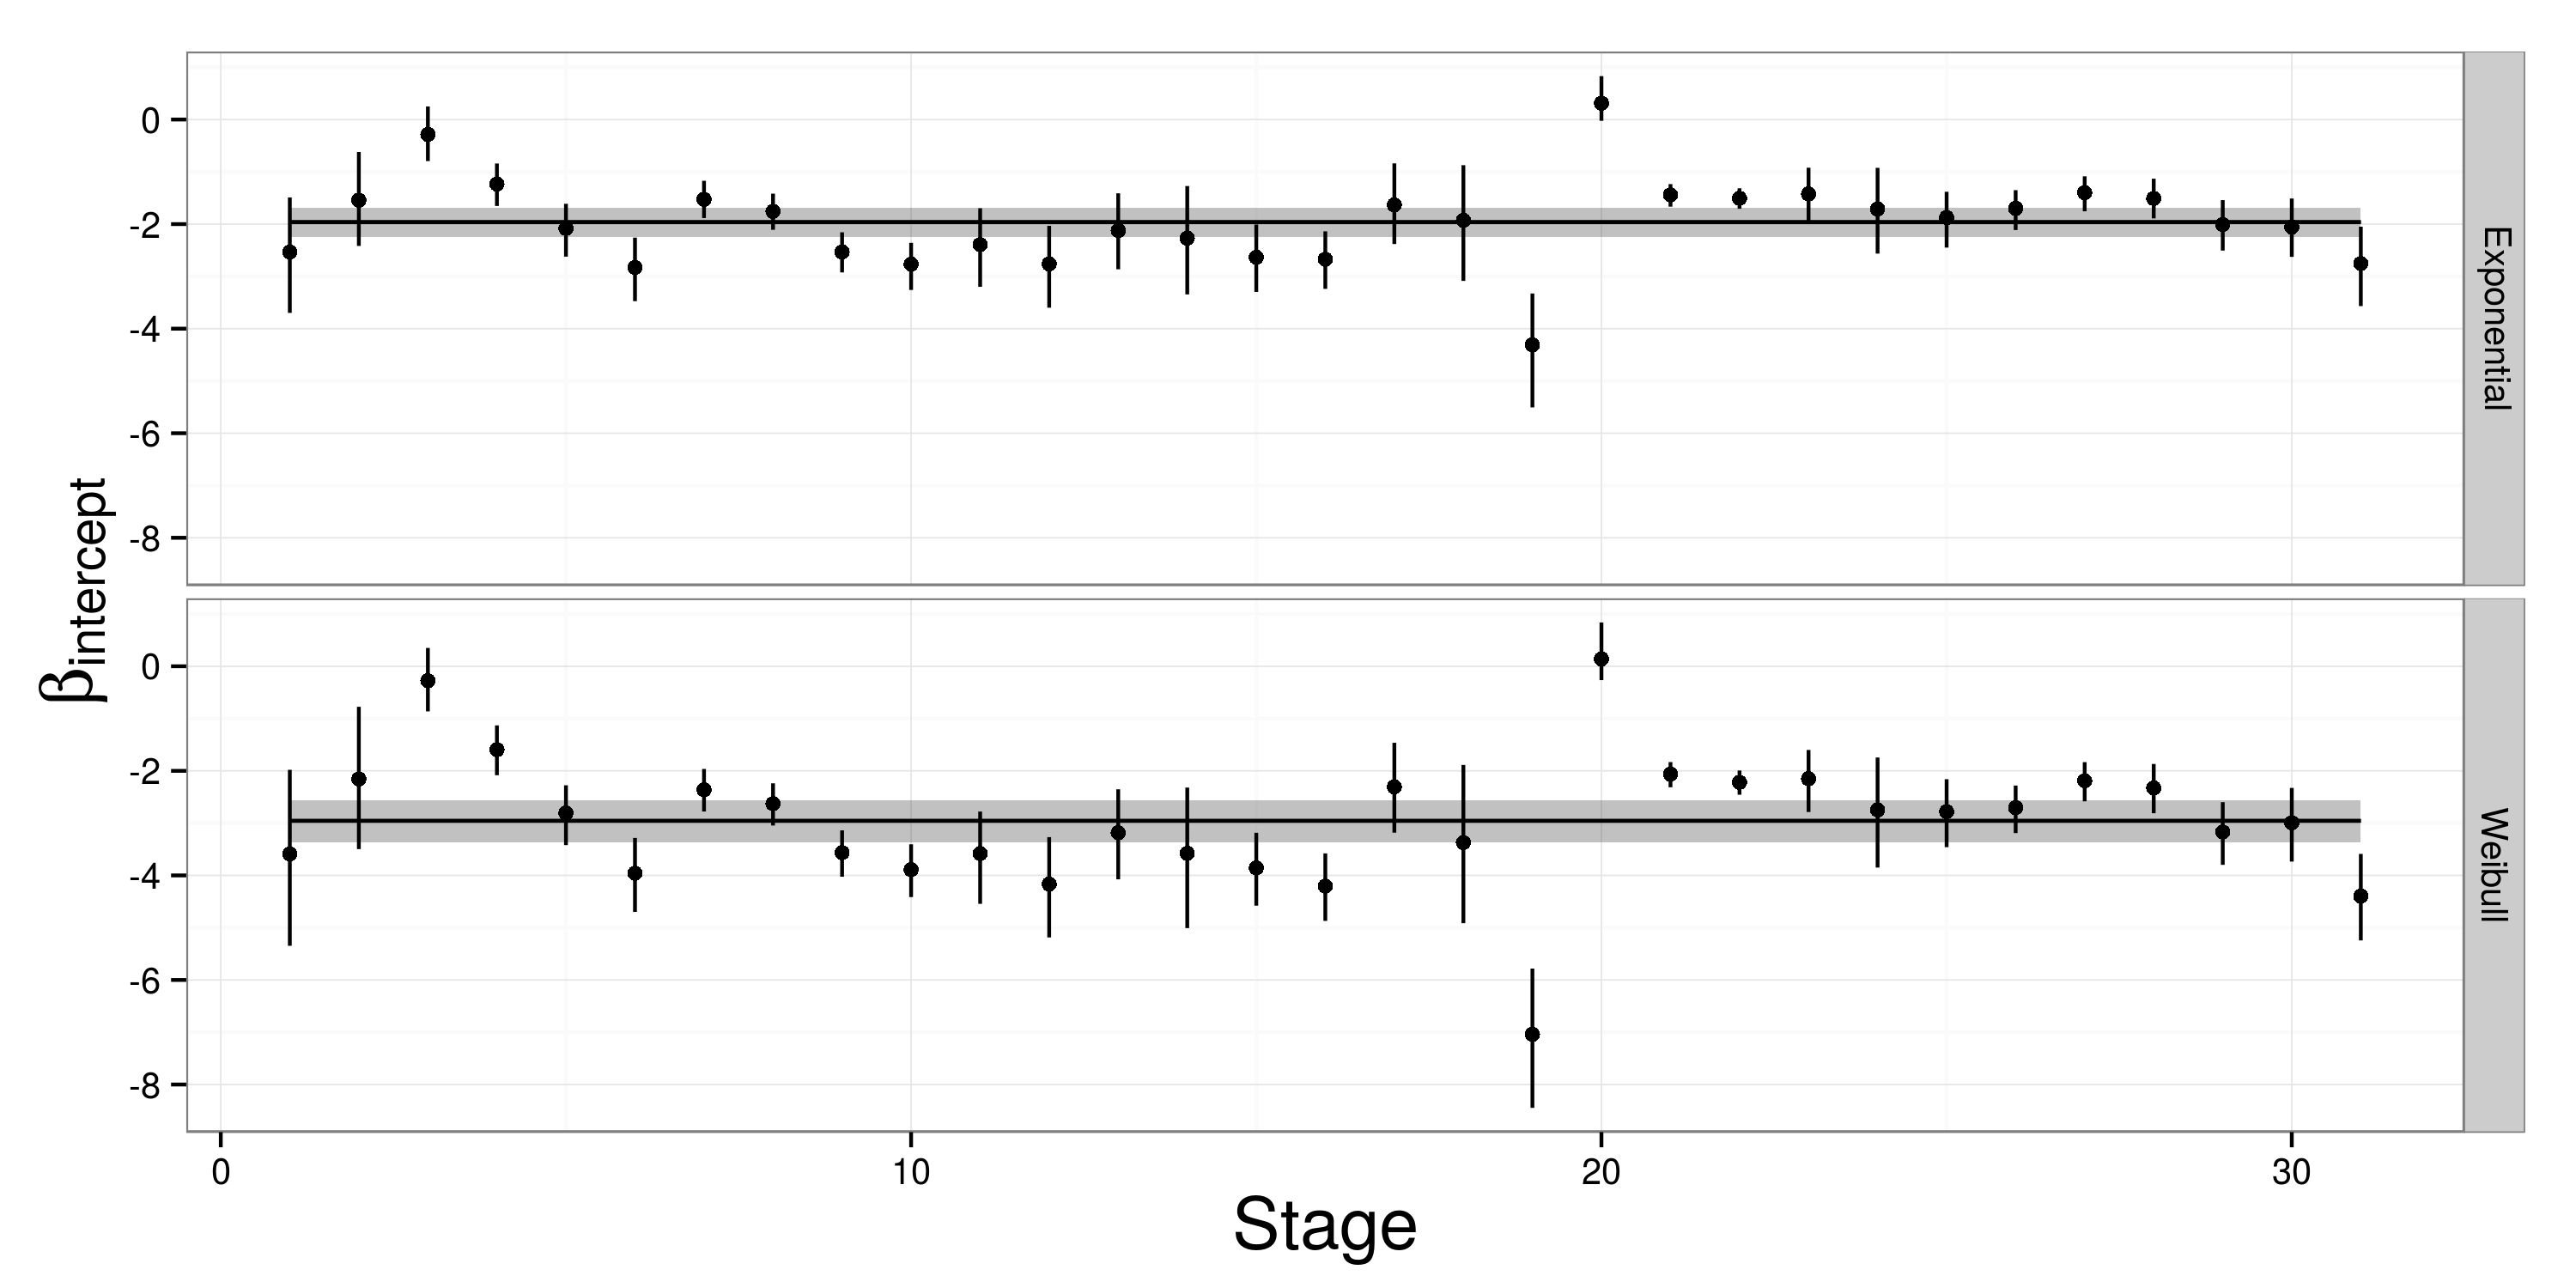
\includegraphics[width = \textwidth,keepaspectratio=true]{figure/intercept_cohort}
    \label{fig:cohort_intercept}
  \end{subfigure}

  \begin{subfigure}[b]{\textwidth}
    \caption{}
    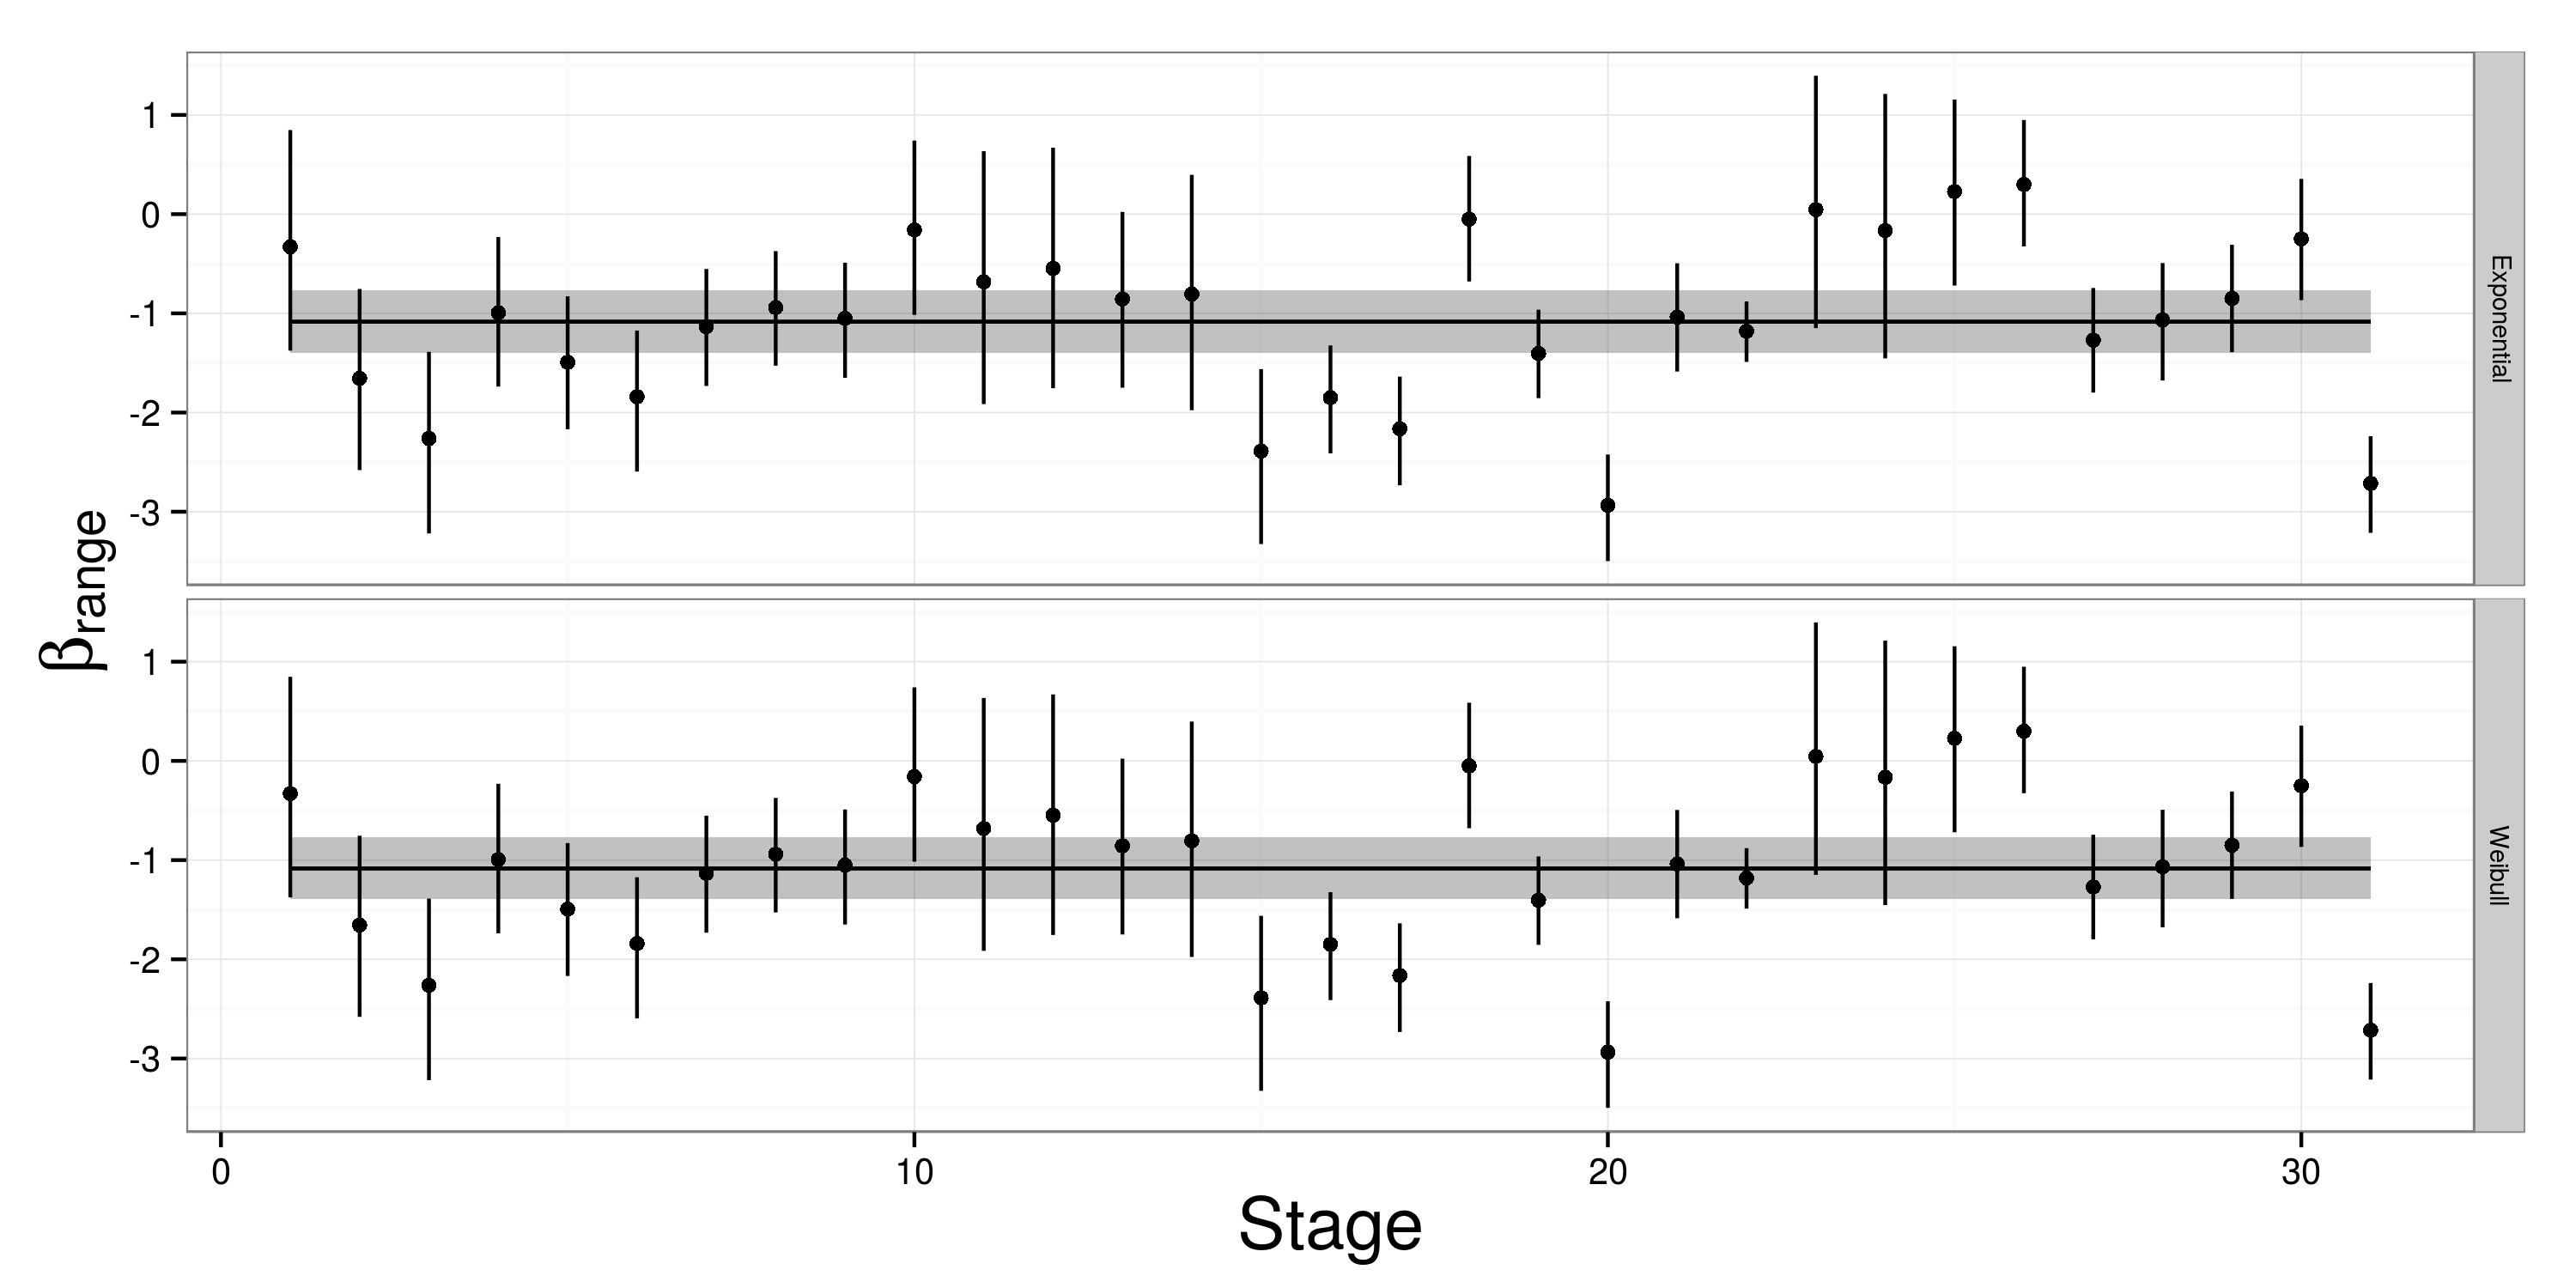
\includegraphics[width = \textwidth,keepaspectratio=true]{figure/range_cohort}
    \label{fig:cohort_range}
  \end{subfigure}
  \caption{Comparison of cohort-specific estimates of \(\beta_{0}\) presented along with the estimate for the overall baseline extinction risk. Points correspond to the median of the cohort-specific estimate, along with 80\% credible intervals. The horizontal line is the median estimate of the overall baseline extinction risk along with 80\% credible intervals. Results are presented for the exponential (top) and Weibull (bottom) models. Comparison of cohort-specific estimates of the effect of geographic range on extinction risk \(\beta_{r}\) presented along with the estimate for the overall effect of geographic range. Points correspond to the median of the cohort-specific estimate, along with 80\% credible intervals. The horizontal line is the median estimate of the overall baseline extinction risk along with 80\% credible intervals. Results are presented for the exponential (top) and Weibull (bottom) models.}
  \label{fig:cohort_info}
\end{figure}


\begin{sidewaysfigure}[ht]
  \centering
  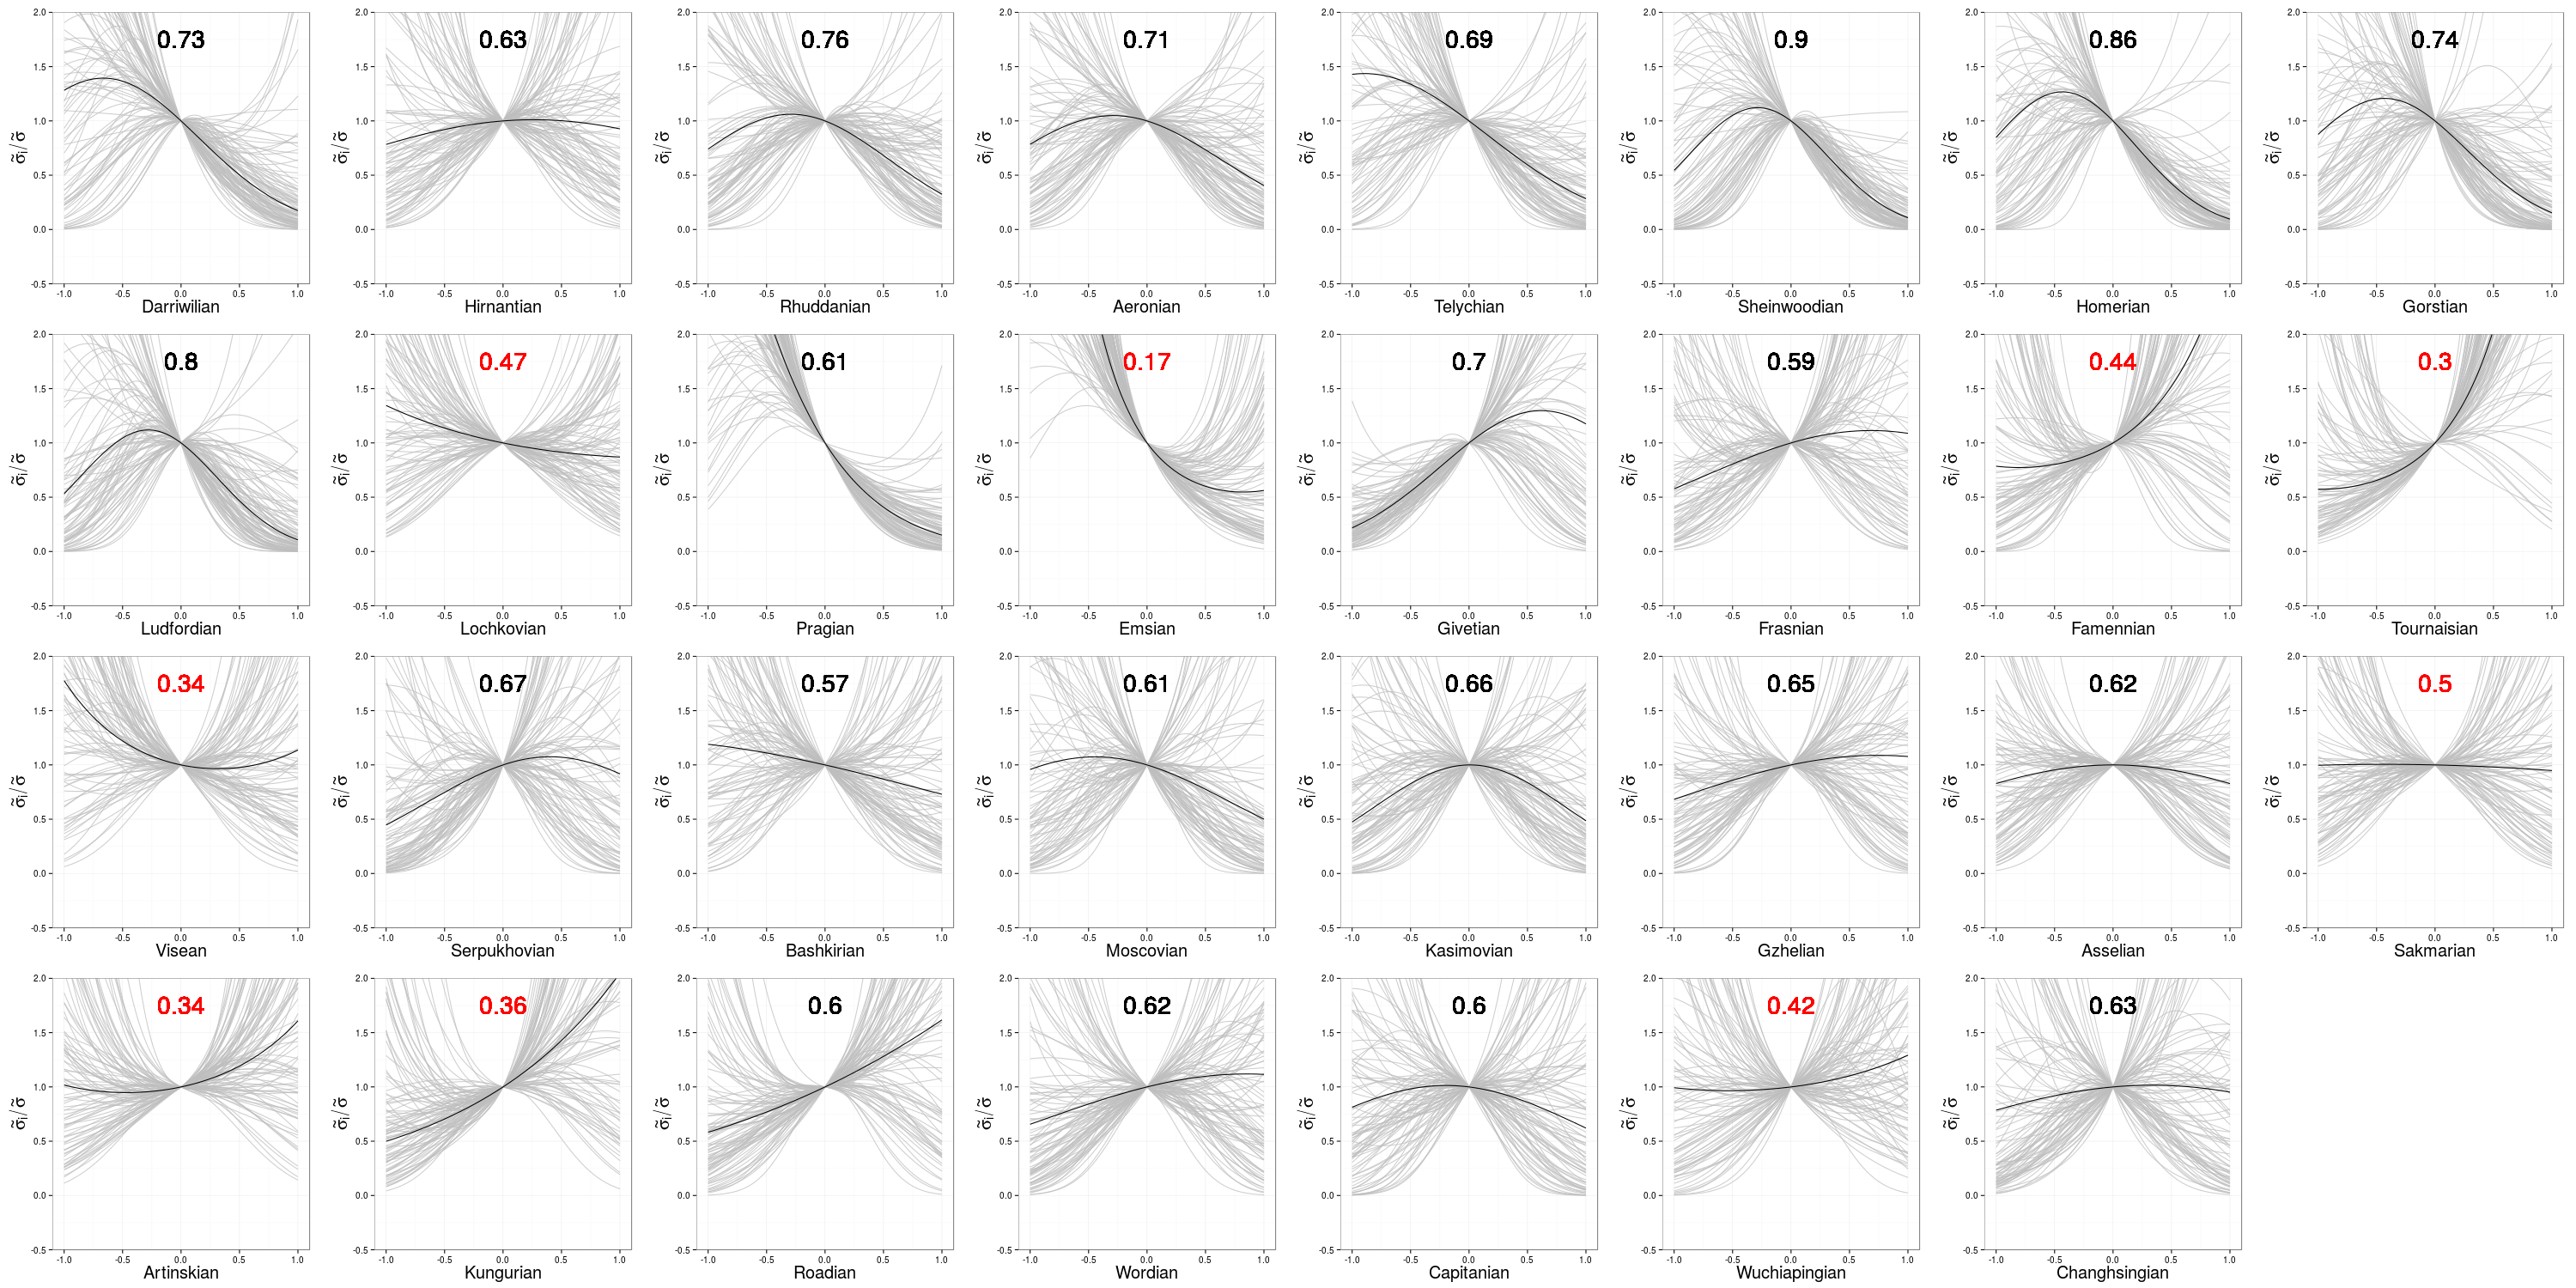
\includegraphics[height = 0.5\textheight,width=\textwidth,keepaspectratio=true]{figure/cohort_quads}
  \caption{Comparison of the cohort-specific estimates of \(f(v_{i})\) (Eq. \ref{eq:env}) for the 33 analyzed origination cohorts. The stage of origination is labeled on the x-axis of each panel. The oldest stage is in the upper left, while the youngest is in the lower left. The number in each panel corresponds to the posterior probability that \(f(v_{i})\) is concave down. Those that are highlighed in red have less than 51\% posterior predictive probability that \(f(v_{i})\) is concave down.}
  \label{fig:env_cohort}
\end{sidewaysfigure}

\begin{table}
  \centering
  \begin{tabular}{ l r r }
    \hline
    parameter & mean & standard deviation \\ 
    \hline
    \(\mu_{i}\) & -1.51 & 0.15 \\ 
    \(\mu_{r}\) & -1.38 & 0.14 \\ 
    \(\mu_{e}\) & -0.08 & 0.18 \\ 
    \(\mu_{e2}\) & 0.25 & 0.43 \\ 
    \(\mu_{m}\) & -0.09 & 0.09 \\ 
    \(\tau_{i}\) & 0.63 & 0.11 \\ 
    \(\tau_{r}\) & 0.48 & 0.12 \\ 
    \(\tau_{e}\) & 1.07 & 0.23 \\ 
    \(\tau_{e^{2}}\) & 1.88 & 0.66 \\ 
    \(\tau_{m}\) & 0.32 & 0.13 \\ 
    \hline
  \end{tabular}
  \caption{<+Caption text+>}
  \label{tab:param}
\end{table}

\end{document}
